\documentclass[tikz,border=4pt]{standalone}
\usepackage{pgfplots}
\usepgfplotslibrary{groupplots}
\pgfplotsset{compat=1.16}
% banda passante in blu, banda attenuata in rosso
\colorlet{bpass}{blue!45}
\colorlet{batt}{red!45}
\pgfplotsset{
  ideale/.style={
    width=4.2cm, height=3.3cm,
    xmode=log, xmin=0.1, xmax=10, xminorticks=false,
    ymin=0, ymax=1.3, ytick={0,1},
    grid=major, major grid style={gray!55},
    tick label style={font=\footnotesize}, label style={font=\small},
    title style={font=\small}, xlabel={$f$},
  },
}
\begin{document}
% Risposte in frequenza IDEALI: |H| lineare, f in scala logaritmica,
% cosi' f0 e' la media geometrica di fL e fH (fL = 0,5, fH = 2, f0 = 1).
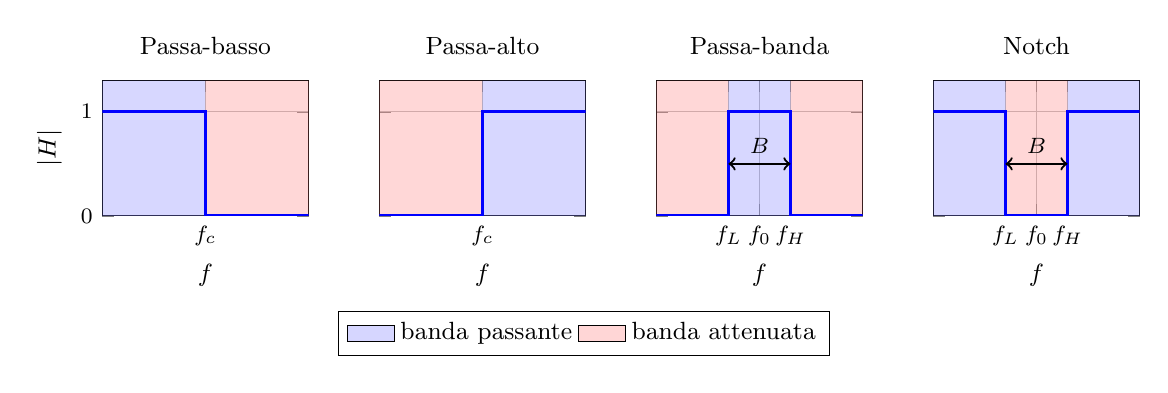
\begin{tikzpicture}
\begin{groupplot}[ideale, group style={group size=4 by 1, horizontal sep=0.9cm,
    y descriptions at=edge left}]

  % ---------- passa-basso ----------
  \nextgroupplot[title={Passa-basso}, ylabel={$|H|$},
    xtick={1}, xticklabels={$f_c$}]
    \addplot[draw=none, fill=bpass, fill opacity=0.35] coordinates {(0.1,0) (0.1,1.3) (1,1.3) (1,0)} \closedcycle;
    \addplot[draw=none, fill=batt, fill opacity=0.35] coordinates {(1,0) (1,1.3) (10,1.3) (10,0)} \closedcycle;
    \addplot[blue, very thick] coordinates {(0.1,1) (1,1) (1,0) (10,0)};

  % ---------- passa-alto ----------
  \nextgroupplot[title={Passa-alto},
    xtick={1}, xticklabels={$f_c$}]
    \addplot[draw=none, fill=batt, fill opacity=0.35] coordinates {(0.1,0) (0.1,1.3) (1,1.3) (1,0)} \closedcycle;
    \addplot[draw=none, fill=bpass, fill opacity=0.35] coordinates {(1,0) (1,1.3) (10,1.3) (10,0)} \closedcycle;
    \addplot[blue, very thick] coordinates {(0.1,0) (1,0) (1,1) (10,1)};

  % ---------- passa-banda ----------
  \nextgroupplot[title={Passa-banda},
    xtick={0.5,1,2}, xticklabels={$f_L$,$f_0$,$f_H$}]
    \addplot[draw=none, fill=batt, fill opacity=0.35] coordinates {(0.1,0) (0.1,1.3) (0.5,1.3) (0.5,0)} \closedcycle;
    \addplot[draw=none, fill=bpass, fill opacity=0.35] coordinates {(0.5,0) (0.5,1.3) (2,1.3) (2,0)} \closedcycle;
    \addplot[draw=none, fill=batt, fill opacity=0.35] coordinates {(2,0) (2,1.3) (10,1.3) (10,0)} \closedcycle;
    \addplot[blue, very thick] coordinates {(0.1,0) (0.5,0) (0.5,1) (2,1) (2,0) (10,0)};
    \draw[<->, thick] (axis cs:0.5,0.5) -- (axis cs:2,0.5)
      node[midway, above, font=\footnotesize] {$B$};

  % ---------- elimina-banda (notch) ----------
  \nextgroupplot[title={Notch},
    xtick={0.5,1,2}, xticklabels={$f_L$,$f_0$,$f_H$},
    legend to name=legideali, legend columns=2, legend style={font=\small},
    legend cell align=left]
    \addplot[draw=none, fill=bpass, fill opacity=0.35, area legend] coordinates {(0.1,0) (0.1,1.3) (0.5,1.3) (0.5,0)} \closedcycle;
    \addlegendentry{banda passante}
    \addplot[draw=none, fill=batt, fill opacity=0.35, area legend] coordinates {(0.5,0) (0.5,1.3) (2,1.3) (2,0)} \closedcycle;
    \addlegendentry{banda attenuata}
    \addplot[draw=none, fill=bpass, fill opacity=0.35, forget plot] coordinates {(2,0) (2,1.3) (10,1.3) (10,0)} \closedcycle;
    \addplot[blue, very thick, forget plot] coordinates {(0.1,1) (0.5,1) (0.5,0) (2,0) (2,1) (10,1)};
    \draw[<->, thick] (axis cs:0.5,0.5) -- (axis cs:2,0.5)
      node[midway, above, font=\footnotesize] {$B$};
\end{groupplot}
\node[anchor=north] at ([yshift=-2pt]current bounding box.south) {\pgfplotslegendfromname{legideali}};
\end{tikzpicture}
\end{document}